\documentclass[a4paper]{article} % use larger type; default would be 10pt
\usepackage[landscape]{geometry}

\usepackage{tikz}

% Tikz initialize
\usetikzlibrary{shapes, arrows, positioning, fit}
\tikzstyle{dashbox} = [rectangle, dashed, draw=black]
\tikzstyle{box} = [rectangle, draw=black, minimum width=2.5cm, minimum height=1cm, text centered, text width=2.5cm]
\tikzstyle{cbox} = [cloud, cloud puffs=15.7, minimum height=1cm, draw]
\tikzstyle{line} = [thin,-,>=stealth]
\tikzstyle{fbox} = [box, dotted, rounded corners=1mm]
\tikzstyle{fcont} = [rectangle, draw=black, minimum width=6cm, minimum height=2.5cm, text centered, text width=6cm]
\tikzstyle{circ} = [circle, draw=black, text centered,  minimum width=2cm, text width=2cm]


\begin{document}
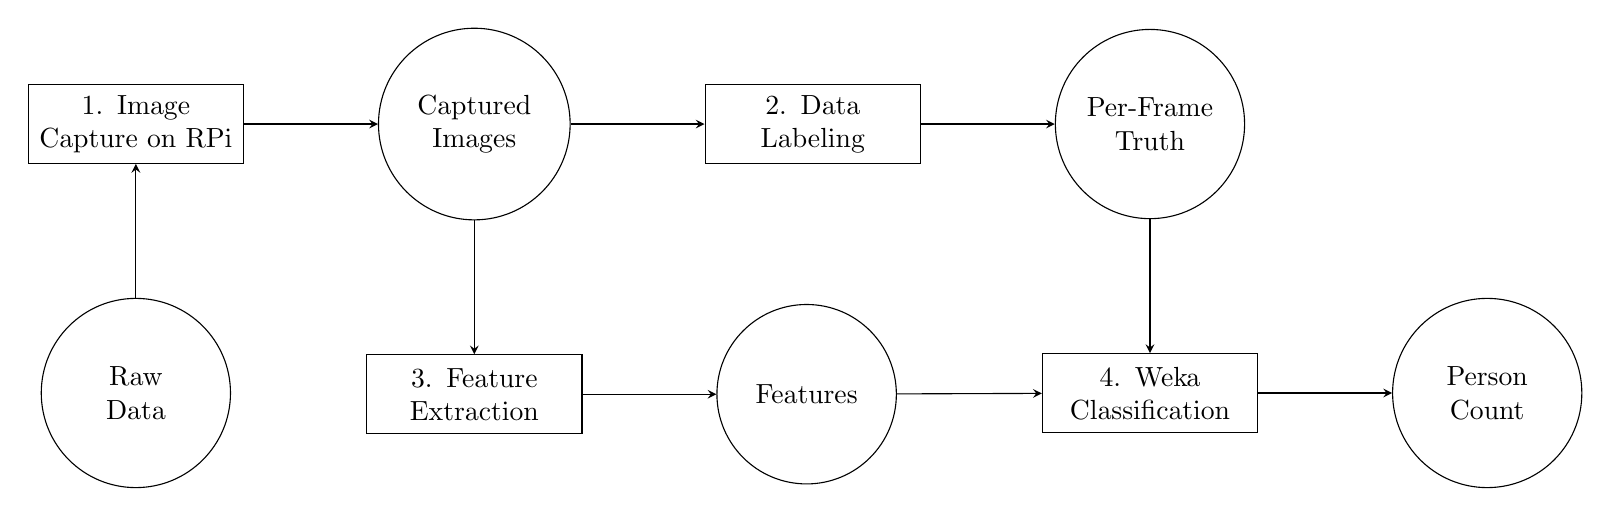
\begin{tikzpicture}[node distance=1.7cm]
\node (raw) [circ] {Raw \linebreak Data};
\node (step1) [box, above=of raw] {1. Image \linebreak Capture on RPi};
\node (frames) [circ, right=of step1] {Captured Images};
\node (step2) [box, right=of frames] {2. Data Labeling};
\node (truth) [circ, right=of step2] {Per-Frame Truth};
\node (step3) [box, below=of frames] {3. Feature Extraction};
\node (csv) [circ, right=of step3] {Features};
\node (step4) [box, below=of truth] {4. Weka Classification};
\node (results) [circ, right=of step4] {Person Count};

\draw [line,->] (raw) -- (step1);
\draw [line,->] (step1) -- (frames);
\draw [line,->] (frames) -- (step2);
\draw [line,->] (step2) -- (truth);
\draw [line,->] (truth) -- (step4);
\draw [line,->] (step3) -- (csv);
\draw [line,->] (csv) -- (step4);
\draw [line,->] (step4) -- (results);

\draw [line,->] (frames) -- (step3);
\end{tikzpicture}
\end{document}
